\section{Two Fundamental Axioms}
\label{sec:two-axioms}

We now discuss two axioms (desirable characteristics) for attribution
methods. We find that other feature attribution methods in literature
break at least one of the two axioms.  These methods include DeepLift~\cite{SGSK16, SGK17},
Layer-wise relevance propagation (LRP)
\cite{BMBMS16}, Deconvolutional networks~\cite{ZF14}, and Guided
back-propagation~\cite{SDBR14}. As we will see in
Section~\ref{sec:method}, these axioms will also guide the design of
our method.

\stitle{Gradients}
For linear models, ML practitioners regularly inspect the products of the
model coefficients and the feature values in order to debug predictions.
Gradients (of the output with respect
to the input) is a natural analog of the model coefficients for a deep network,
and therefore the product of the gradient and feature values  is a reasonable
starting point for an attribution method ~\cite{BSHKHM10, SVZ13}; see the third column of
Figure~\ref{fig:intgrad-finalgrad} for examples. The problem with
gradients is that they break \emph{sensitivity}, a property
that all attribution methods should satisfy.

\subsection{Axiom: Sensitivity(a)} An attribution method satisfies \emph{Sensitivity(a)}
if for every input and baseline that differ in one feature but have different
predictions then the differing feature should be given a non-zero attribution.
(Later in the paper, we will have a part (b) to this definition.)

Gradients violate Sensitivity(a): For a concrete example, consider a
one variable, one ReLU network, $f(x) = 1 - \relu(1-x)$.  Suppose the
baseline is $x=0$ and the input is $x=2$. The function changes from $0$ to
$1$, but because $f$ becomes flat at $x=1$, the gradient method gives
attribution of $0$ to $x$.  Intuitively, gradients break Sensitivity
because the prediction function may flatten at the input and thus have
zero gradient despite the function value at the input being different
from that at the baseline. This phenomenon has been reported in
previous work~\cite{SGSK16}.

Practically, the lack of sensitivity causes gradients to focus on
irrelevant features (see the ``fireboat'' example in
Figure~\ref{fig:intgrad-finalgrad}).

\stitle{Other back-propagation based approaches} A second set of approaches
involve back-propagating the final prediction score through each layer
of the network down to the individual features.  These include
DeepLift, Layer-wise relevance propagation (LRP), Deconvolutional networks (DeConvNets),
and Guided back-propagation. These methods differ in
the specific backpropagation logic for various activation functions
(e.g., ReLU, MaxPool, etc.).

Unfortunately, Deconvolution networks (DeConvNets), and
Guided back-propagation violate Sensitivity(a).
This is because these methods back-propogate through a ReLU node
only if the ReLU is turned on at the input. This makes the method
similar to gradients, in that, the attribution is zero for features
with zero gradient at the input despite a non-zero gradient at the
baseline. We defer the specific counterexamples to Appendix~\ref{sec:examples}.

Methods like DeepLift and LRP tackle the Sensitivity issue by
employing a baseline, and in some sense try to compute ``discrete
gradients'' instead of (instantaeneous) gradients at the input.
(The two methods differ in the specifics of how they compute the discrete gradient).
But the idea is that a large, discrete step will avoid flat regions, avoiding a
breakage of sensitivity.  Unfortunately, these methods violate a
different requirement on attribution methods.

\subsection{Axiom: Implementation Invariance} Two networks are \emph{functionally
equivalent} if their outputs are equal for all inputs, despite
having very different implementations. Attribution
methods should satisfy \emph{Implementation Invariance}, i.e., the
attributions are always identical for two functionally equivalent
networks.  To motivate this, notice that attribution can be
colloquially defined as assigning the blame (or credit) for the
output to the input features. Such a definition does not refer to
implementation details.
%% Moreover, the common practice of machine
%% learning tends to evaluate the models from an input-output point of
%% view, where implementations are purely means to an end.

We now discuss intuition for why DeepLift and LRP break Implementation
Invariance; a concrete example is provided in Appendix~\ref{sec:examples}.

First, notice that gradients are invariant to implementation.
In fact, the chain-rule for
gradients $\frac{\partial f}{\partial g}=\frac{\partial f}{\partial
  h}\cdot \frac{\partial h}{\partial g}$ is essentially about
implementation invariance. To see this, think of $g$ and $f$ as the input
and output of a system, and $h$ being some implementation detail of the
system.  The gradient of output $f$ to input $g$
can be computed either directly by $\frac{\partial f}{\partial g}$,
ignoring the intermediate function $h$ (implementation detail), or by
invoking the chain rule via $h$. This is exactly how backpropagation works.
Methods like LRP and DeepLift replace gradients with discrete
gradients and still use a modified form of backpropagation to compose
discrete gradients into attributions.
Unfortunately, the chain rule does not hold for discrete gradients in
general. Formally
$\frac{f(x_1)-f(x_0)}{g(x_1)-g(x_0)}\neq\frac{f(x_1)-f(x_0)}{h(x_1)-h(x_0)}\cdot\frac{h(x_1)-h(x_0)}{g(x_1)-g(x_0)}$
, and therefore these methods fail to satisfy implementation invariance.

If an attribution method fails to satisfy Implementation Invariance,
the attributions are potentially sensitive to unimportant aspects of
the models.
For instance, if the network architecture has more degrees of freedom
than needed to represent a function then there may be two sets of values
for the network parameters that lead to the same function.
%% For instance, in the example in the appendix,
%% the network architecture has more degrees of freedom than needed for
%% representing the function, and as a result there are two set of values
%% for the network parameters that lead to the same function.
%For instance, in the example in Section~\ref{sec:examples},
%the two networks have more degree of freedom than needed for representing
%the same function.
The training procedure can converge at either set of values depending
on the initializtion or for other reasons, but the underlying network
function would remain the same. It is undesirable that attributions differ
for such reasons.


\section{Our Method: Integrated Gradients}
\label{sec:method}


We are now ready to describe our technique. Intuitively, our technique
combines the Implementation Invariance of Gradients along with the Sensitivity
of techniques like LRP or DeepLift.

Formally, suppose we have a
function $F: \reals^n \rightarrow [0,1]$ that represents a deep network.
Specifically, let $x \in \reals^n$ be the input at hand, and
$\xbase \in \reals^n$ be the baseline input. For image networks, the baseline
could be the black image, while for text models it could be the zero
embedding vector.

We consider the straightline path (in $\reals^n$) from the baseline $\xbase$ to the input
$x$, and compute the gradients at all points along the path. Integrated gradients
are obtained by cumulating these gradients. Specifically, integrated gradients
are defined as the path intergral of the gradients along the straightline
path from the baseline $\xbase$ to the input $x$.

The integrated gradient along the $i^{th}$ dimension for an input $x$ and baseline
$\xbase$ is defined as follows. Here,
$\tfrac{\partial F(x)}{\partial x_i}$ is the gradient of
$F(x)$ along the $i^{th}$ dimension.
\begin{equation}
\small
\integratedgrads_i(x) \synteq (x_i-\xbase_i)\times\int_{\sparam=0}^{1} \tfrac{\partial F(\xbase + \sparam\times(x-\xbase))}{\partial x_i  }~d\sparam
\end{equation}
 
\stitle{Axiom: Completeness}
Integrated gradients satisfy an axiom called \emph{completeness}
that the attributions add
up to the difference between the output of $F$ at the input
$x$ and the \emph{baseline}
$\xbase$. 

This axiom is identified as being desirable by Deeplift and LRP.
It is a sanity check that the attribution method is somewhat comprehensive
in its accounting, a property that is clearly desirable if the network’s score is
used in a numeric sense, and not just to pick the top label, for e.g.,
a model estimating insurance premiums from credit features of individuals.

This is formalized by the proposition below, which
instantiates the fundamental theorem of calculus for path
integrals.
\begin{proposition}\label{prop:additivity}
  If $F: \reals^n \rightarrow \reals$ is differentiable almost
  everywhere
  \footnote{Formally, this means the function $F$ is continuous everywhere
    and the partial derivative of $F$ along each input dimension satisfies
    Lebesgue's integrability condition, i.e., the set of discontinuous points
    has measure zero. Deep networks built out of Sigmoids, ReLUs, and pooling
    operators satisfy this condition.} then
  $$\Sigma_{i=1}^{n} \integratedgrads_i(x) = F(x) -
  F(\xbase)$$
\end{proposition}

For most deep networks, it is possible to choose a baseline such that
the prediction at the baseline is near zero ($F(\xbase) \approx
0$). (For image models, the black image baseline indeed satisfies
this property.) In such cases, there is an intepretation of the resulting
attributions that ignores the baseline and amounts to distributing the
output to the individual input features.

\begin{remark}\label{rem:compsens}
  Integrated gradients satisfies Sensivity(a) because Completeness implies
Sensivity(a) and is thus a strengthening of the Sensitivity(a) axiom. This
is because Sensitivity(a) refers to a case where the baseline and the input
differ only in one variable, for which Completeness asserts that the difference
in the two output values is equal to the attribution to this variable.
Attributions generated by integrated gradients satisfy Implementation Invariance
since they are based only on the gradients of the function represented
by the network.
\end{remark}

%% The final input along this path is the input for which we need the input. The first input in this path is the benchmark.

%% and a set of counterfactual inputs falling on a path in $\reals^n$.






%% The additivity property provides a form of sanity checking for the integrated
%% gradients and ensures that we do not under or over attribute to
%% features. This is a common pitfall for attribution schemes based on
%% feature ablations, wherein, an ablation may lead to small or a large change in
%% the prediction score depending on whether the ablated feature
%% interacts disjunctively or conjunctively to the rest of the features.
%% This additivity is even more desirable when the network’s score is
%% numerically critical, i.e., the score is not used purely in an ordinal
%% sense. In this case, the attributions (together with additivity)
%% guarantee that the attributions are in the \emph{units} of the score,
%% and account for all of the score.








%% TODO(mukunds): make shorter, make description general (input is specified as an embedding).





%% The gradient tensor for each value of $\sparam$ is in the space of the
%% input, and can be visualized by overlaying it on the original
%% input. For image classification networks, the gradients can be
%% visualized by scaling pixel intesities in the actual image in
%% proportion to their corresponding
%% gradients. Figure~\ref{fig:camera-intgrads} shows the visualizations
%% for an image classified as ``reflex camera'' for various values of the
%% scaling parameter $\sparam$. The visualizations show how the
%% importance of each pixel evolves as we scale the image, with the last
%% visualization being identical to one generated by gradients at the
%% actual image. In this regard, the interior gradients offer strictly
%% more insight into pixel importance than just the gradients at the
%% actual image.

%% The plot in the top right
%% corner shows the trend in the absolute magnitude of the average pixel
%% importance score. The magnitude is significantly larger at lower
%% values of $\sparam$ and nearly zero at higher values --- the latter is
%% a consequence of saturation.
%% Note that each visualization is only
%% indicative of the relative distribution of the importance scores
%% across pixels and not the absolute magnitude of the scores, i.e., the
%% later snapshots are responsible for tiny increases in the scores as
%% the chart in the top right depicts.
%%
%% Why this may be the case? When the scaling parameter is very small (or
%% equivalently the brightness is very low), only the distinctive
%% patterns in the image are visible. Consequently, the network only
%% focusses on them. As the image is scaled up, we speculate that two
%% things happen - (1) Subtle and less distinctive patterns gain
%% visibility, and (2) Saturation increases in the network.  We further
%% posit that neurons responsible for the distinctive features move into
%% saturation, thereby dropping the gradients for those features. This is
%% why the interior gradients at high values of the scaling parameter
%% depict seemingly insignificant patterns.
%

%% \begin{figure}[!htb]
%%   \begin{center}
%%     \begin{subfigure}{.5\columnwidth}
%%       \centering
%%       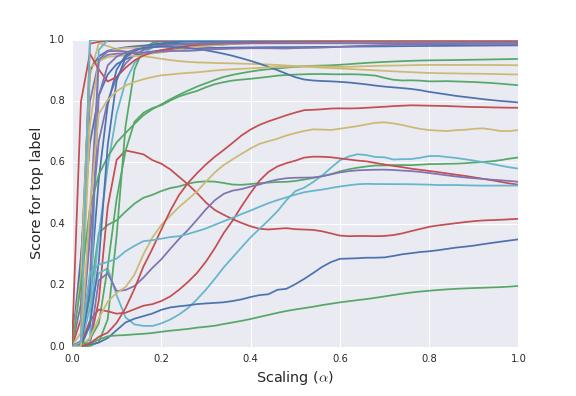
\includegraphics[width=0.8\columnwidth]{./Figures/Saturation/smax.jpg}
%%       \caption{Softmax score for top label}\label{fig:sat-incp-smax}
%%     \end{subfigure}%
%%     \begin{subfigure}{.5\columnwidth}
%%       \centering
%%       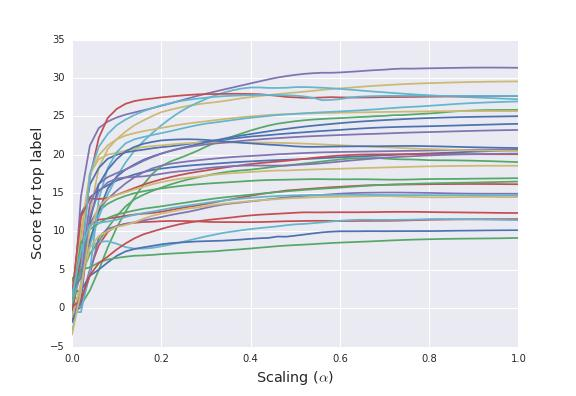
\includegraphics[width=0.8\textwidth]{./Figures/Saturation/smax_pre.jpg}
%%       \caption{Pre-softmax score for top label}\label{fig:sat-incp-presmax}
%%     \end{subfigure}
%%   %\fbox{\rule[-.5cm]{0cm}{4cm} \rule[-.5cm]{4cm}{0cm}}
%%   \end{center}
%%   \caption{Saturation in Inception}\label{fig:sat-incp}
%% \end{figure}

%% \begin{figure}
%%   \centering
%%   %% \begin{subfigure}{0.9\columnwidth}
%%   %%   \centering
%%   %%   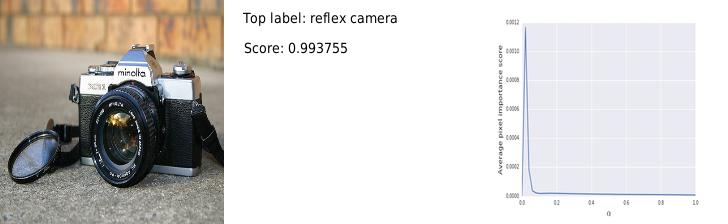
\includegraphics[width=0.9\textwidth]{./Figures/Gifs/CameraGifImages/camera-curve.jpg}
%%   %%   \caption*{Input image and trend of the pixel importance scores
%%   %%     obtained from interior gradients.}
%%   %%   \vspace{0.5cm}
%%   %% \end{subfigure}
%%   \begin{subfigure}{.2\columnwidth}
%%     \centering
%%     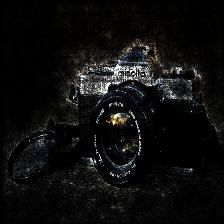
\includegraphics[width=0.9\columnwidth]{./Figures/Gifs/CameraGifImages/camera-1.jpg}
%%     \caption*{$\alpha= 0.02$}
%%   \end{subfigure}%
%%   \begin{subfigure}{.2\columnwidth}
%%     \centering
%%     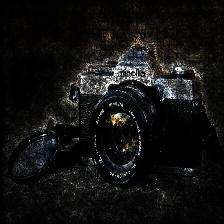
\includegraphics[width=0.9\columnwidth]{./Figures/Gifs/CameraGifImages/camera-2.jpg}
%%     \caption*{$\alpha= 0.04$}
%%   \end{subfigure}%
%%   \begin{subfigure}{.2\columnwidth}
%%     \centering
%%     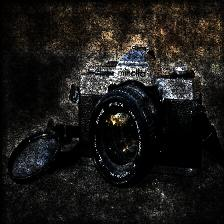
\includegraphics[width=0.9\columnwidth]{./Figures/Gifs/CameraGifImages/camera-3.jpg}
%%     \caption*{$\alpha= 0.06$}
%%   \end{subfigure}%
%%   \begin{subfigure}{.2\columnwidth}
%%     \centering
%%     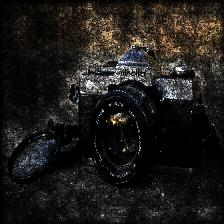
\includegraphics[width=0.9\columnwidth]{./Figures/Gifs/CameraGifImages/camera-4.jpg}
%%     \caption*{$\alpha= 0.08$}
%%   \end{subfigure}
%%   \begin{subfigure}{.2\columnwidth}
%%     \centering
%%     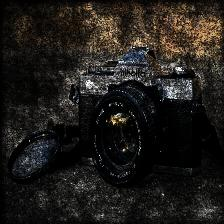
\includegraphics[width=0.9\columnwidth]{./Figures/Gifs/CameraGifImages/camera-5.jpg}
%%     \caption*{$\alpha= 0.1$}
%%   \end{subfigure}%
%%   \begin{subfigure}{.2\columnwidth}
%%     \centering
%%     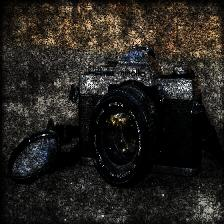
\includegraphics[width=0.9\columnwidth]{./Figures/Gifs/CameraGifImages/camera-10.jpg}
%%     \caption*{$\alpha= 0.2$}
%%   \end{subfigure}%
%%   \begin{subfigure}{.2\columnwidth}
%%     \centering
%%     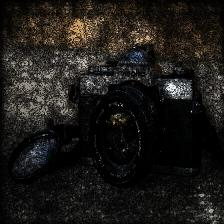
\includegraphics[width=0.9\columnwidth]{./Figures/Gifs/CameraGifImages/camera-20.jpg}
%%     \caption*{$\alpha= 0.4$}
%%   \end{subfigure}%
%%   \begin{subfigure}{.2\columnwidth}
%%     \centering
%%     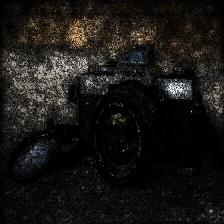
\includegraphics[width=0.9\columnwidth]{./Figures/Gifs/CameraGifImages/camera-30.jpg}
%%     \caption*{$\alpha= 0.6$}
%%   \end{subfigure}
%%   \begin{subfigure}{.2\columnwidth}
%%     \centering
%%     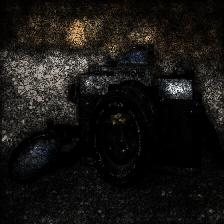
\includegraphics[width=0.9\columnwidth]{./Figures/Gifs/CameraGifImages/camera-40.jpg}
%%     \caption*{$\alpha= 0.8$}
%%   \end{subfigure}%
%%   \begin{subfigure}{.2\columnwidth}
%%     \centering
%%     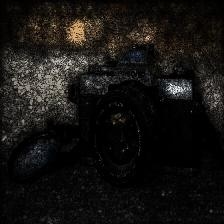
\includegraphics[width=0.9\columnwidth]{./Figures/Gifs/CameraGifImages/camera-50.jpg}
%%     \caption*{$\alpha= 1.0$}
%%   \end{subfigure}
%%   \caption{\textbf{Visualization of interior gradients.} Notice that the visualizations at
%%     lower values of the scaling parameter ($\alpha$) are sharper and much better at surfacing
%%     important features of the input image.}
%%   \label{fig:camera-intgrads}
%% \end{figure}

%% \subsection{Cumulating Interior Gradients}
%% Interior gradients can be summarized by integrating them along the path
%% $\pathfn(\alpha)$ for $\alpha \in [0, 1]$. We call the resulting gradients as
%% \emph{\bf integrated gradients}. While there are a few ways of
%% cumulating counterfactual gradients, the approach we take has the nice
%% \emph{attribution} property (Proposition~\ref{prop:additivity}) that
%% the feature importance scores approximately add up to the prediction
%% score. The feature importance scores are thus also referred to as
%% \emph{attributions}.

%% Formally, the integrated gradient along the $i^{th}$ dimension for an input $x \in \reals^n$
%% is defined as follows.
%% \begin{equation}
%% \integratedgrads_i(x) \synteq \int_{\sparam=0}^{1} \tfrac{\partial F(\pathfn(\sparam))}{\partial \pathfn_i(\sparam)  }~\tfrac{\partial \pathfn_i(\sparam)}{\partial \sparam}  ~d\sparam
%% \end{equation}
%% where $\tfrac{\partial F(x)}{\partial x_i}$ is the gradient of
%% $F$ along the $i^{th}$ dimension at $x$.

%% A nice technical property of the integrated gradients is that they add
%% up to the difference between the output of $F$ at the final
%% counterfactual $\pathfn(1)$ and the \emph{baseline} counterfactual
%% $\pathfn(0)$.  This is formalized by the proposition below, which is
%% an instantiation of the fundamental theorem of calculus for path
%% integrals.
%% \begin{proposition}\label{prop:additivity}
%%   If $F: \reals^n \rightarrow \reals$ is differentiable almost
%%   everywhere
%%   \footnote{Formally, this means that the partial derivative of $F$
%%     along each input dimension satisfies Lebesgue's integrability
%%     condition, i.e., the set of discontinuous points has measure
%%     zero. Deep networks built out of Sigmoids, ReLUs, and pooling
%%     operators should satisfy this condition.}, and $\pathfn: [0,1]
%%   \rightarrow \reals^n$ is smooth then
%%   $$\Sigma_{i=1}^{n} \integratedgrads_i(x) = F(\pathfn(1)) -
%%   F(\pathfn(0))$$
%% \end{proposition}

%% For most deep networks, it is possible to choose counterfactuals such
%% that the prediction at the baseline counterfactual is near zero
%% ($F(\pathfn(0)) \approx 0$).\footnote{We did have trouble finding a
%%    baseline couterfactual for an RNN model that simulated the workings of
%%    a traffic light intersection between a main road and a side street;
%%    the naive benchmark counterfactual was one of no traffic at either
%%    intersection. But this did not have the lack of semantics that a
%%    black image or pure noise has for the Inception network. While no
%%    interesting labels are activated for the black image supplied to
%%    the Inception network, the same is not true for the ``no traffic''
%%    benchmark supplied to the RNN model.}
%% For instance, for image classification networks, the prediction at the
%% black image baseline is neutral, i.e., nearly zero for all classes.
%% In such cases. In such cases, it follows from the Proposition that the integrated
%% gradients form an attribution of the prediction output $F(x)$, i.e.,
%% they almost exactly distribute the output to the individual input features.


%% Integrated Gradients (ignoring the approximation in computing
%% integrals) satisfies Sensitivity.  The attribution to the variable is
%% in fact equal to the change in function value (this is a one-variable
%% instance of Proposition~\ref{prop:additivity}).


%% \todo(mukunds): Move the following paragraph elsewhere.



%% \subsection{Rationale}
%% While measuring saturation via counterfactuals seems natural, using
%% them for quantifying feature importance deserves some discussion. The
%% first thing one may try to identify feature importance is to examine
%% the deep network like one would with human authored code. This seems
%% hard; just as deep networks employ distributed
%% representations (such as embeddings), they perform convoluted (pun
%% intended) distributed reasoning. So instead, we choose to probe the
%% network with several counterfactual inputs (related to the input at
%% hand), hoping to trigger all the internal workings of the network.
%% This process would help summarize the effect of the network on the
%% protagonist input; the assumption being that the input is human
%% understandable. Naturally, it helps to work with
%% gradients in this process as via back propagation, they induce an
%% aggregate view over the function computed by the neurons.

%% Interior gradients use counterfactual inputs to artifactually induce a
%% procedure on how the network’s attention moves across the image as it
%% compute the final prediction score. From the animation, we gather that the
%% network focuses on strong and distinctive patterns in the image at
%% lower values of the scaling parameter, and subtle and weak patterns in
%% the image at higher values.  Thus, we speculate that the network's
%% computation can be loosely abstracted by a procedure that first
%% recognize distinctive features of the image to make an initial
%% prediction, and then fine tunes (these are small score jumps as
%% the chart in Figure~\ref{fig:camera-intgrads} shows) the prediction
%% using weaker patterns in the image.


%% \section{Saturation}
%% TODO(mukunds): move this to the two axioms section

%% \subsection{Gradients Do Not Reflect Feature Importance}
%% Let us start by investigating the performance of gradients as a measure of feature importance.
%% We use an object recognition network built using the GoogleNet
%% architecture (\cite{SLJSRAEVR14}) as a running example; we refer to this
%% network by its codename Inception. (We present applications of our
%% techniques to other networks in Section~\ref{sec:beyond-inception}.)
%% The network has been trained on the ImageNet object recognition
%% dataset (\cite{ILSVRC15}). It is is $22$ layers deep with a softmax layer on top for
%% classifying images into one of the $1000$ ImageNet object classes.
%% The input to the
%% network is a $224 \times 224$ sized RGB image.

%% Before evaluating the use of gradients for feature importance, we introduce some basic notation that is used throughout
%% the paper.

%% We represent a $224\times 224$ sized RGB image as a vector in
%% $\reals^{224\times 224\times 3}$. Let $\incp^L: \reals^{224\times 224\times 3} \rightarrow [0,1]$ be
%% the function represented by the Inception network that computes the
%% softmax score for the object class labeled $L$.
%% %\footnote{While we explain the technique with respect to the
%% %  highest scoring object class, it can be applied to any specific
%% %  object class}
%% Let $\grad\incp^L(\img)$ be the gradients of $\incp^L$
%%  at the input
%% image $\img$. Thus, the vector $\grad\incp^L(\img)$ is the same size as
%% the image and lies in $\reals^{224\times 224\times 3}$.  As a shorthand, we write
%% $\grad\incp^L_{i,j,c}(\img)$ for the gradient of a specific pixel
%% $(i,j)$ and color channel $c \in \{R,G,B\}$.

%% We compute the gradients of $\incp^L$ (with respect to the image) for the
%% highest-scoring object class, and then aggregate the gradients $\grad\incp^L(\img)$
%% along the color dimension to obtain pixel importance scores.\footnote{
%%   These pixel importance scores are similar to the gradient-based
%%   saliency map defined by~\cite{SVZ13} with the
%%   difference being in how the gradients are aggregated along the color
%%   channel.}
%% \begin{equation}\label{eq:pimportance}
%% \forall i, j: \pimportance^L_{i,j}(\img)  ~\synteq~  \Sigma_{c \in \{R,G,B\}} \vert\grad\incp^L_{i,j,c}(\img)\vert
%% \end{equation}
%% Next, we visualize pixel importance scores by scaling the intensities of the
%% pixels in the original image in proportion to their respective scores;
%% thus, higher the score brighter would be the pixel. Figure
%% \ref{fig:camera-finalgrad} shows a visualization for an
%% image for which the highest scoring object class is ``reflex camera''
%% with a softmax score of $0.9938$.

%% \begin{figure}
%%   \begin{center}
%%     \begin{subfigure}{.9\columnwidth}
%%       \centering
%%       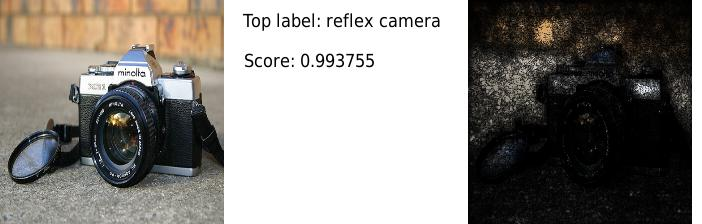
\includegraphics[width=0.9\columnwidth]{./Figures/FinalGrad/camera.jpg}
%%       \caption{Original image.}\label{fig:camera-finalgrad}
%%     \end{subfigure}
%%     \begin{subfigure}{.9\columnwidth}
%%       \centering
%%       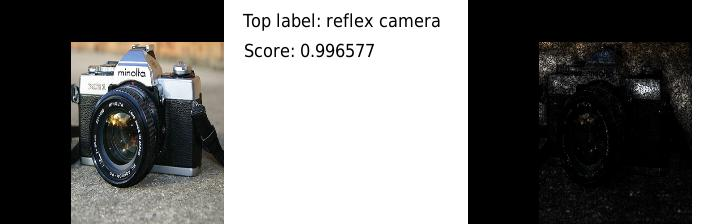
\includegraphics[width=0.9\columnwidth]{./Figures/FinalGrad/camera_ablation.jpg}
%%       \caption{Ablated image.}\label{fig:camera-abl-finalgrad}
%%     \end{subfigure}
%%     %\fbox{\rule[-.5cm]{0cm}{4cm} \rule[-.5cm]{4cm}{0cm}}
%%   \end{center}
%%   \caption{Pixel importance using gradients at the image.}
%% \end{figure}

%% Intuitively, one would expect the the high gradient pixels for this
%% classification to be ones falling on the camera or those providing
%% useful context for the classification (e.g., the lens cap). However,
%% most of the highlighted pixels seem to be on the left or above the
%% camera, which to a human seem not essential to the prediction. This could
%% either mean that (1) the highlighted pixels are somehow important for
%% the internal computation performed by the Inception network, or (2)
%% gradients of the image fail to appropriately quantify pixel
%% importance.

%% Let us consider hypothesis (1). In order to test it we ablate parts of
%% the image on the left and above the camera (by zeroing out the pixel
%% intensities) and run the ablated image through the Inception
%% network. See Figure~\ref{fig:camera-abl-finalgrad}. The top
%% predicted category still remains ``reflex camera'' with a softmax
%% score of $0.9966$ --- slightly higher than before. This indicates that
%% the ablated portions are indeed irrelevant to the classification. On
%% computing gradients of the ablated image, we still find that most of
%% the high gradient pixels lie outside of the camera.  This suggests
%% that for this image,  it is in fact hypothesis (2) that holds true.
%% Upon studying more images (see Figure~\ref{fig:intgrad-finalgrad}), we find that
%% the gradients often fail to highlight the relevant pixels for the predicted
%% object label.

%% \subsection{Saturation}\label{sec:saturation}
%% In theory, it is easy to see that the gradients may not reflect
%% feature importance if the prediction function flattens in the vicinity
%% of the input, or equivalently, the gradient of the prediction function
%% with respect to the input is tiny in the vicinity of the input vector. This
%% is what we call \emph{saturation}, which has also been reported in previous
%% work (\cite{SGSK16},~\cite{GB10}).

%% We analyze how widespread saturation is in the Inception network by
%% inspecting the behavior of the network on \textbf{counterfactual images}
%% obtained by uniformly scaling pixel intensities from zero to their
%% values in an actual image. Formally, given an input image $\im \in \reals^{224\times 224\times 3}$,
%% the set of counterfactual images is
%% \begin{equation}
%% \{\sparam~\im~\vert~ 0 \leq \sparam \leq 1\}
%% \end{equation}
%% Figure~\ref{fig:sat-incp-smax} shows the trend in the softmax output of the
%% highest scoring class, for thirty randomly chosen images form the ImageNet
%% dataset. More specifically, for each image $\im$, it shows the trend in
%% $\incp^L(\sparam~\im)$ as $\sparam$ varies from zero to one with $L$ being
%% the label of highest scoring object class for $\im$. It is easy to
%% see that the trend flattens (saturates) for all images
%% $\sparam$ increases. Notice that saturation is present even for images whose
%% final score is significantly below $1.0$. Moreover, for a majority of images,
%% saturation happens quite soon when $\sparam=0.2$.

%% One may argue that since the output of the Inception network is the result of
%% applying the softmax function to a vector of activation values,
%% the saturation is expected due to the squashing property of the softmax function.
%% However, as shown in Figure~\ref{fig:sat-incp-presmax}, we find that even the
%% pre-softmax activation scores for the highest scoring class saturate.

%% In fact, to our surprise, we found that the saturation is inherently present
%% in the Inception network and the outputs of the intermediate layers also
%% saturate. We plot the distance between the intermediate layer neuron activations
%% for a scaled down input image and the actual input image with respect to the
%% scaling parameter, and find that the trend flattens. Due to lack of space, we
%% provide these plots in Figure~\ref{fig:sat-incp-intermediate} in the appendix.

%% It is quite clear from these plots that saturation is widespread
%% across images in the Inception network, and there is a lot more
%% activity in the network for counterfactual images at relatively low
%% values of the scaling parameter $\sparam$. This observation forms the basis of our
%% technique for quantifying feature importance.

%% Note that it is well known that the saturation of gradients prevent
%% the model from converging to a good quality minima (\cite{GB10}). So one
%% may expect good quality models to not have saturation and hence for
%% the (final) gradients to convey feature importance. Clearly, our observations on the
%% Inception model show that this is not the case. It has good prediction
%% accuracy, but also exhibits saturation (see Figure~\ref{fig:sat-incp}).
%% Our hypothesis is that the gradients of important features are
%% \emph{not} saturated early in the training process. The gradients only
%% saturate \emph{after} the features have been learned adequately, i.e.,
%% the input is far away from the decision boundary.





